\section{问题三的模型与求解}

\subsection{附件3的预测质量与信息到达}

附件3每日在 0:00、6:00、12:00 和 18:00 发布未来24个整点的光伏功率预测。令发布时间为 $\tau$，第 $h$ 个预测值的目标时刻定义为
\[
t^{\mathrm{tar}}=\tau+h,\qquad h=1,\ldots,24.
\]
原始数据共包含1460个发布批次和35040个小时预测节点，所有批次均具有完整的24个提前期，且不存在重复键、负预测值和非整点目标。年末36个目标时刻超出附件2的实测范围，评价时保留其来源记录但不强行匹配。

为适配10分钟运行网格，本文在每个发布批次内部采用PCHIP插值，原始小时节点保持不变，且不跨批次借用信息。表\ref{tab:q3-official-lead}表明，官方预测误差随提前期显著扩大：1--3 h的MAE为34.52 kW，而19--24 h增至319.51 kW。因此，后续预测融合需要显式区分提前期。

\begin{table}[H]
\centering
\small
\caption{附件3官方光伏预测的提前期误差}
\label{tab:q3-official-lead}
\begin{tabular}{lrrrr}
\toprule
提前期 & 样本数 & MAE/kW & RMSE/kW & 偏差/kW \\
\midrule
1-3h & 4380 & 34.52 & 69.43 & 0.62 \\
4-6h & 4380 & 77.78 & 170.45 & -3.57 \\
7-12h & 8754 & 144.79 & 298.88 & -16.13 \\
13-18h & 8748 & 226.29 & 458.91 & -39.59 \\
19-24h & 8742 & 319.51 & 673.02 & -65.92 \\
\bottomrule
\end{tabular}
\end{table}


\begin{figure}[H]
  \centering
  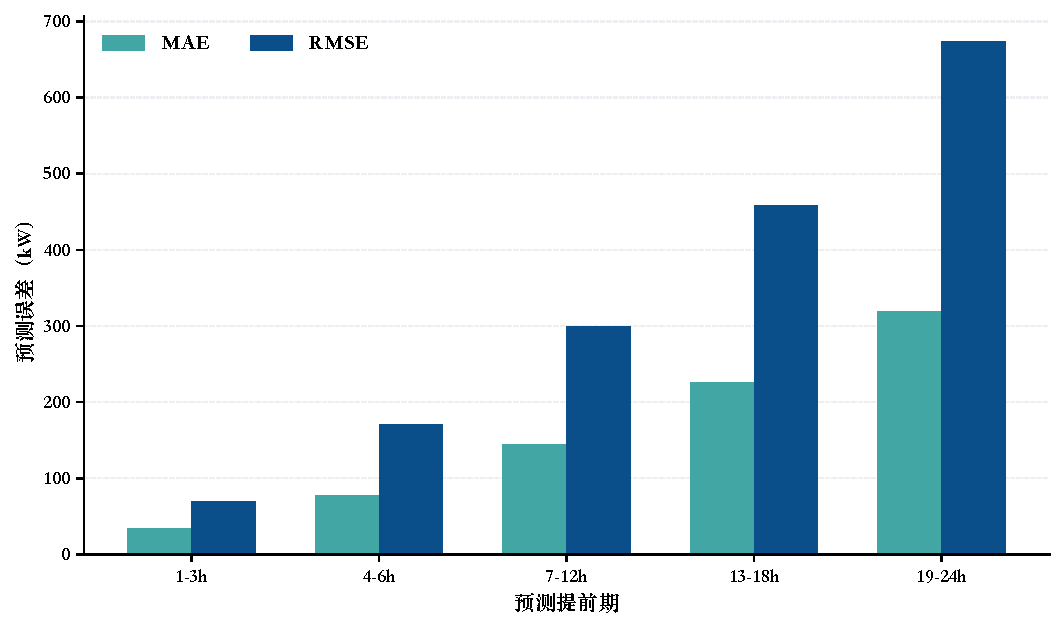
\includegraphics[width=0.78\textwidth]{../results/problem3/figures/fig_p3_official_error_by_lead.pdf}
  \caption{附件3官方光伏预测误差随提前期的变化}
  \label{fig:q3-official-lead}
\end{figure}

\subsection{因果预测融合}

候选预测包括官方预测、昨日同刻、上周同刻和七日同刻均值。先用2025年1月8日至16日拟合融合权重，再用1月17日至30日完成模型选择，2月1日至12月31日作为正式样本外评价期。该划分以发布时间归属运营日，确保正式评价开始前已完成全部模型选择。

验证结果选择七日同刻均值作为季节性专家。进一步令 $w_b$ 表示提前期分箱 $b$ 内官方预测的权重，则融合预测为
\[
\widehat P_{\tau,h}=w_b\widehat P^{\mathrm{off}}_{\tau,h}+(1-w_b)\widehat P^{\mathrm{sea}}_{\tau,h},
\qquad 0\le w_b\le1.
\]
五个分箱的官方权重依次为0.871、0.450、0.232、0.033和0.089。短提前期主要依赖新发布的官方预测，长提前期则主要依赖较稳定的季节性估计。表\ref{tab:q3-method-comparison}显示，提前期分箱融合的样本外MAE与RMSE分别为121.73 kW和252.99 kW，优于静态融合、按发布时间分组融合和因果在线融合。

\begin{table}[H]
\centering
\small
\caption{问题三候选光伏预测方法的样本外比较}
\label{tab:q3-method-comparison}
\begin{tabular}{lrrrr}
\toprule
方法 & 样本数 & MAE/kW & RMSE/kW & 偏差/kW \\
\midrule
官方预测 & 32028 & 191.83 & 447.97 & -32.39 \\
七日同刻均值 & 32028 & 153.86 & 305.44 & 2.81 \\
静态凸融合 & 32028 & 139.29 & 276.92 & -1.53 \\
提前期分箱融合 & 32028 & 121.73 & 252.99 & -0.81 \\
发布时间分组融合 & 32028 & 132.19 & 265.56 & -1.28 \\
在线因果融合 & 32028 & 153.86 & 305.44 & 2.81 \\
\bottomrule
\end{tabular}
\end{table}


所有预测权重只使用已经完成并获得真值的历史目标更新。改变任一发布时间之后的实际光伏序列，不会改变该时刻已发布的预测。现有结构化预测专家未覆盖四个发布批次的同一整点协议，无法进行公平比较，因此未纳入正式模型。

\subsection{多发布时间更新接口}

本文定义四种信息时间表
\[
S_0=\{0\},\quad S_1=\{0,6\},\quad
S_2=\{0,6,12\},\quad S_3=\{0,6,12,18\}.
\]
在时刻 $\tau$ 到达新预测后，$[0,\tau]$ 内已经执行的区间保持冻结，仅对 $(\tau,24]$ 内的未来区间开放修订。当前实际SOC作为必需的外部状态传入，不能用计划SOC或固定6000 kWh替代。

每次更新均沿用问题二的50条成对负荷--光伏残差场景，并在新的融合光伏预测附近重新居中；场景数、残差来源日和负荷预测机制保持不变。风险参数固定为$\lambda=0$，从而四种安排的差异只来自信息到达时刻。

\subsection{滚动优化、物理执行与调整结算}

设时刻$\tau$以前的当前承诺为$g_t^{\mathrm{old}}$，更新后的承诺为$g_t^{\mathrm{new}}$。对尚未执行的区间定义
\[
g_t^{\mathrm{new}}-g_t^{\mathrm{old}}=\Delta g_t^+-\Delta g_t^- ,
\qquad \Delta g_t^+,\Delta g_t^-\ge 0.
\]
00:00的完整计划仍按问题二的期望成本模型制定。其后的更新把已经支付的原承诺视为沉没成本，在剩余时域最小化
\[
 \sum_{t>\tau}p_t\Delta t
 \left(1.5\Delta g_t^+-0.5\Delta g_t^-\right)
 +\frac1{50}\sum_{s=1}^{50}\sum_{t>\tau}5p_te_{t,s}\Delta t
 -V(E_{145}),
\]
其中$V(E_{145})$是问题二已锁定的分段线性延续价值。该目标与题设结算一致：增购按$1.5p_t$支付，减购仅返还$0.5p_t$。

每次求解后只执行至下一个信息发布时间。实际充、放电动作以计划动作为上限，并调用问题二相同的物理结算：
\[
0\le c_t^{\mathrm{act}}\le c_t^{\mathrm{plan}},\qquad
0\le d_t^{\mathrm{act}}\le d_t^{\mathrm{plan}},
\]
\[
E_{t+1}^{\mathrm{act}}=E_t^{\mathrm{act}}
+0.9c_t^{\mathrm{act}}\Delta t
-\frac{d_t^{\mathrm{act}}\Delta t}{0.9}.
\]
实际放电不超过负荷缺口，未使用的计划电与光伏弃电分别核算，不设置隐藏上网或未吸收放电通道。下一时刻优化使用当前实际SOC，下一日初值等于上一日实际终值。

多次调整的主结果采用“相对上一承诺”逐次结算。由于题目文字也可能理解为所有调整均相对00:00原计划，本文另给出该口径的敏感性结果；两种方式不混合使用。
结果表中的调整购电量是各次增购量与减购量绝对值之和，即gross adjustment；调整费用则是$1.5p_t$增购支出与$0.5p_t$减购返还相抵后的净结算额。因此，调整电量较大而净调整费用较小并不矛盾。

\subsection{年度经济结果与信息价值}

对2025年2月1日至12月31日共334天进行逐日滚动回测，四种信息安排的全部日模型均获得Optimal解。表\ref{tab:q3-schedule-comparison}区分了00:00计划费用、调整费用、实际紧急购电费用和实际总费用；模型内部的场景期望成本不作为实际结算费用。

\begin{table}[H]
\centering\small
\caption{不同信息安排下的年度实际经济结果}
\label{tab:q3-schedule-comparison}
\begin{tabular}{lrrrrr}
\toprule
安排 & 计划费用/万元 & 调整费用/万元 & 紧急费用/万元 & 总费用/万元 & 紧急电量/万kWh \\
\midrule
S0 & 1333.536 & 0.000 & 139.261 & 1472.797 & 36.635 \\
S1 & 1334.358 & 2.274 & 126.654 & 1463.285 & 33.229 \\
S2 & 1334.392 & 0.143 & 116.015 & 1450.550 & 30.225 \\
S3 & 1334.503 & 0.088 & 116.181 & 1450.772 & 30.236 \\
\bottomrule
\end{tabular}
\end{table}


随着6:00和12:00预测加入，紧急购电量由$36.635$万kWh依次降至$33.229$万kWh和$30.225$万kWh，总费用由$1472.797$万元降至$1450.550$万元。18:00更新后总费用为$1450.772$万元，略高于$S_2$。这说明更晚的信息仍会改变承诺，但其减少紧急购电的收益不足以覆盖调整成本及调度变化，故没有必要机械地使用每一次发布。

定义实际经济意义下的信息价值为
\[
\mathrm{VOI}(S_i)=C(S_0)-C(S_i),
\]
而相邻安排的增量价值为$C(S_{i-1})-C(S_i)$。结果见表\ref{tab:q3-voi}。6:00和12:00信息分别贡献$95120.802$元和$127349.063$元的增量价值，18:00信息的增量价值为$-2217.413$元。负值未经截断，反映其在本次事后回测中的真实经济表现；本文不把这一结果表述为事前参数选择。

\begin{table}[H]
\centering\small
\caption{滚动信息的年度价值}
\label{tab:q3-voi}
\begin{tabular}{lrr}
\toprule
安排 & 相对S0的VOI/元 & 新增发布时间的增量VOI/元 \\
\midrule
S0 & 0.000 & 0.000 \\
S1 & 95120.802 & 95120.802 \\
S2 & 222469.865 & 127349.063 \\
S3 & 220252.452 & -2217.413 \\
\bottomrule
\end{tabular}
\end{table}


表\ref{tab:q3-settlement-sensitivity}给出两种结算解释。二者只改变会计口径，不改变计划、实际电池动作、紧急购电量或SOC轨迹。对于$S_2$和$S_3$，两种口径下年度总费用差异均不足600元，信息时刻选择的主要结论保持不变。

\begin{table}[H]
\centering\small
\caption{多次调整结算解释的敏感性结果}
\label{tab:q3-settlement-sensitivity}
\begin{tabular}{llrr}
\toprule
安排 & 结算解释 & 调整费用/元 & 实际总费用/万元 \\
\midrule
S2 & 相对上一承诺 & 1433.572 & 1450.550 \\
S2 & 相对00:00承诺 & 918.047 & 1450.499 \\
S3 & 相对上一承诺 & 879.452 & 1450.772 \\
S3 & 相对00:00承诺 & 363.449 & 1450.720 \\
\bottomrule
\end{tabular}
\end{table}


逐时审计表明，四种安排的实际功率平衡和SOC递推最大残差分别不超过$1.82\times10^{-12}$ kW与$2.28\times10^{-13}$ kWh；跨日SOC残差为0，未吸收放电为0，已执行区间冻结残差为0。正式附件\texttt{result3.xlsx}采用$S_3$，完整保存00:00计划、各更新后的最终承诺、实际充放电与全部10分钟紧急购电记录；是否采用18:00更新的经济判断由上述VOI分析单独给出。
